\documentclass[tikz,border=12pt]{standalone}
\usepackage{fontspec}
\newfontfamily\hebrewfont[Script=Hebrew]{Noto Serif Hebrew}
\newcommand{\heb}[1]{{\hebrewfont #1}}
\newfontfamily\igfont[Ligatures=TeX]{Noto Serif}
\newcommand{\igtext}[1]{{\igfont #1}}
\usepackage{amsmath,amssymb}
\usetikzlibrary{positioning,arrows,shapes,fit,calc,decorations.pathreplacing,backgrounds}

\begin{document}
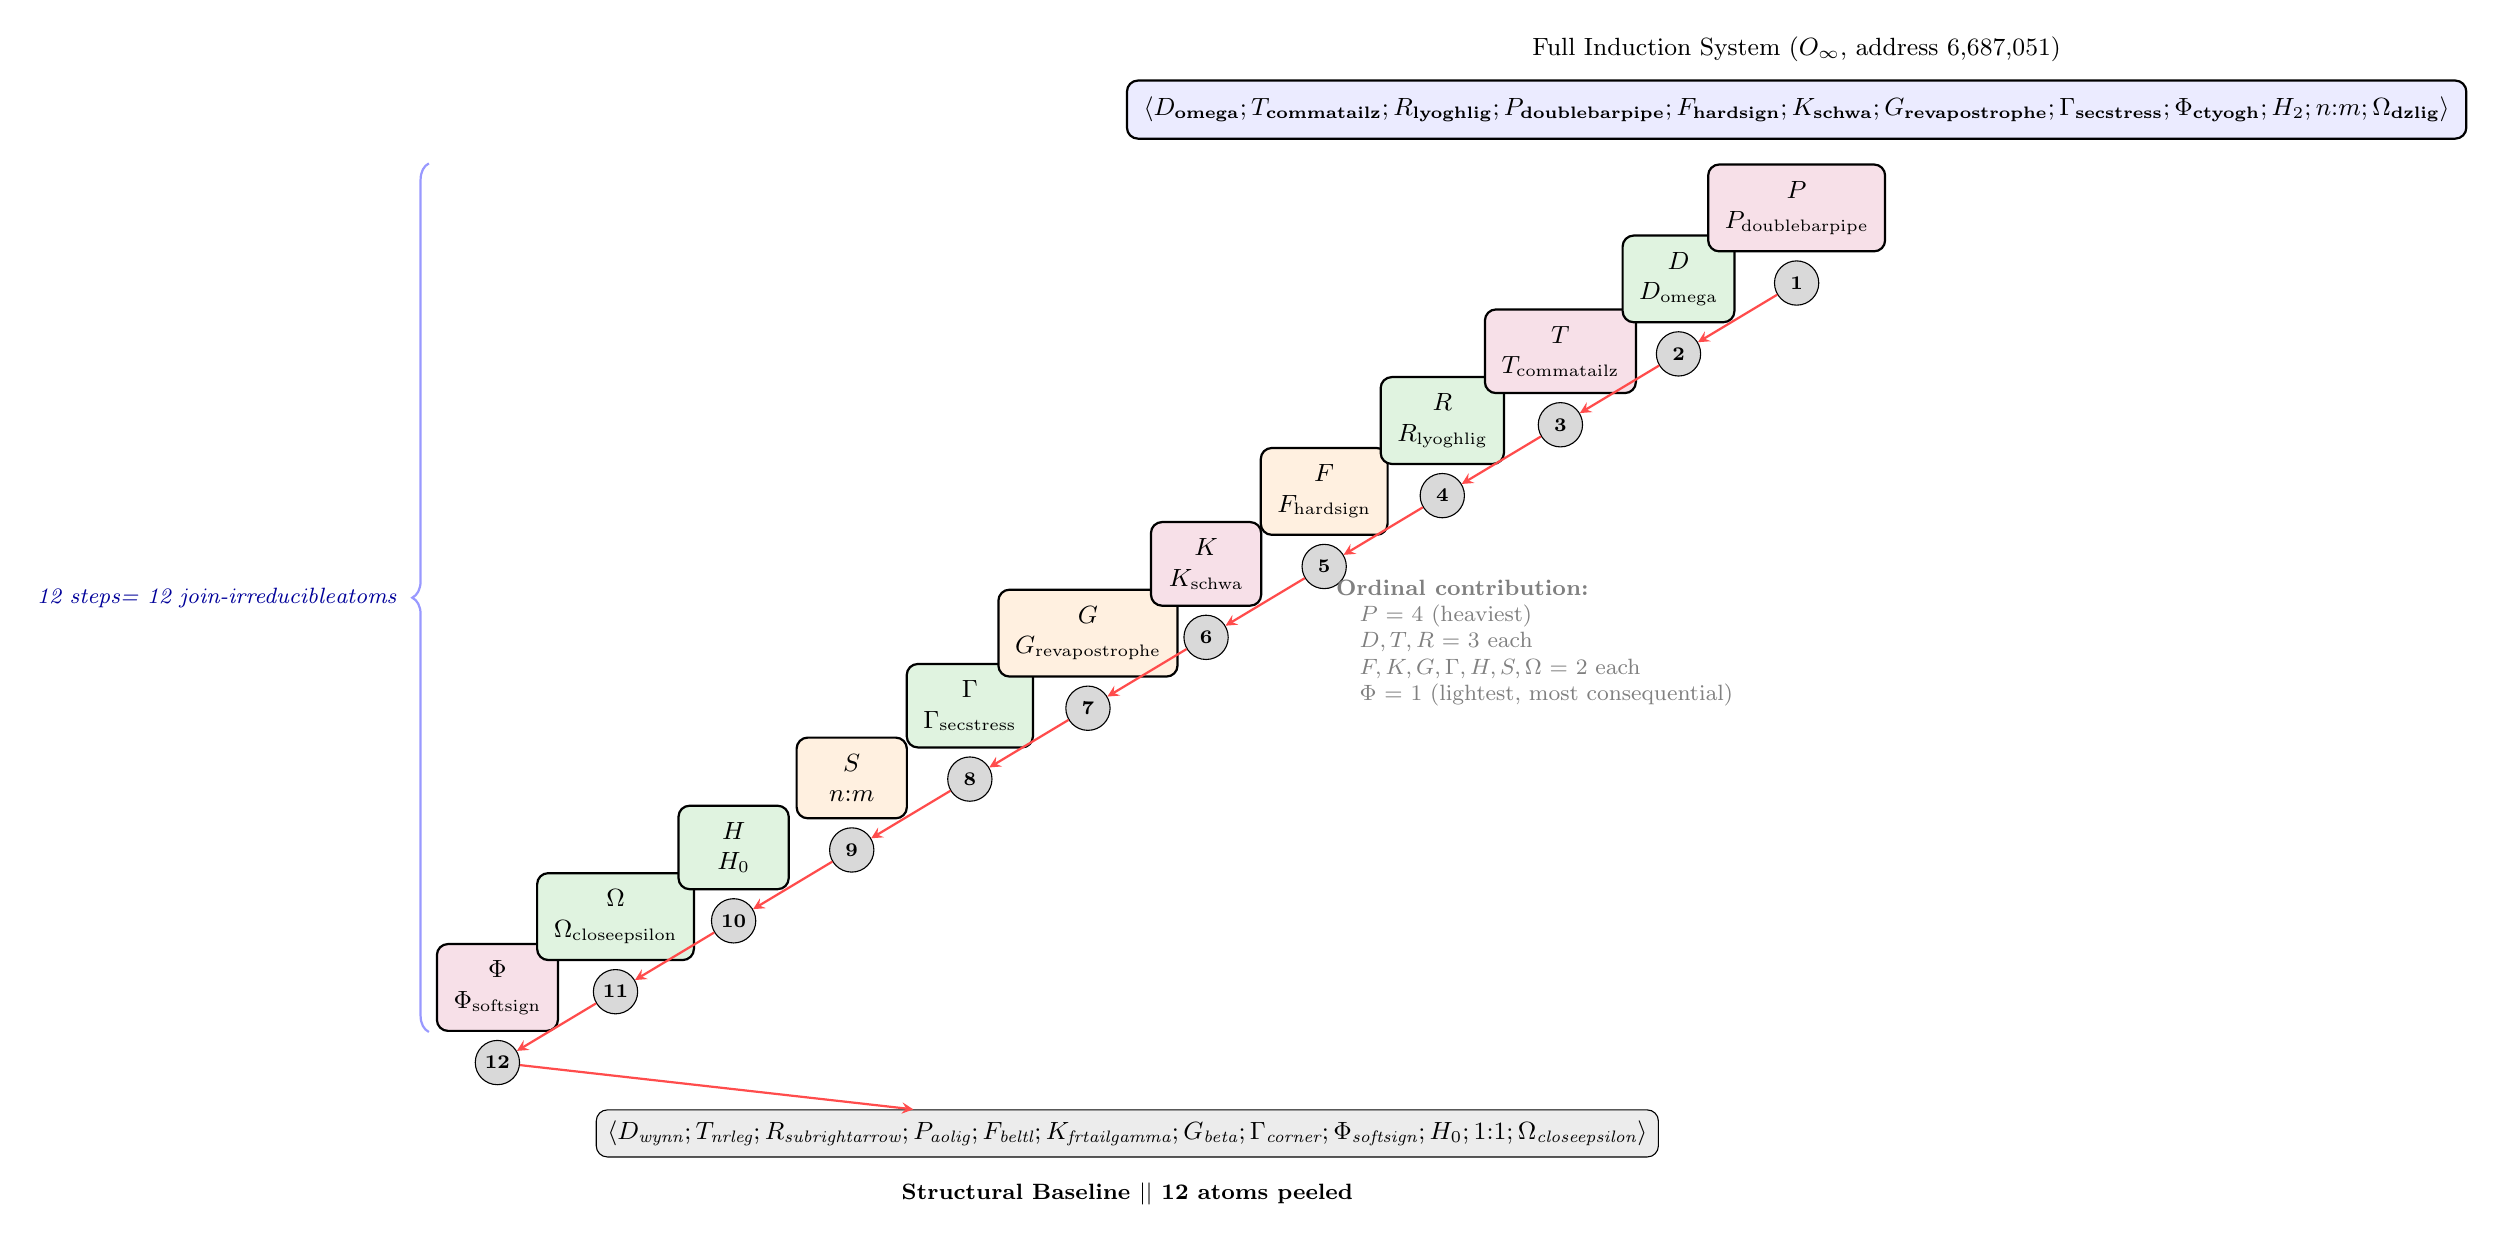
\begin{tikzpicture}[
  prim/.style={rectangle,draw,thick,rounded corners,fill=#1!12,inner sep=6pt,align=center,minimum width=1.4cm,font=\small},
  stepno/.style={circle,draw,fill=gray!30,inner sep=0pt,minimum size=16pt,font=\scriptsize\bfseries},
  peel/.style={->,>=stealth,thick,red!70},
  peellab/.style={font=\footnotesize,fill=white,inner sep=1pt,text=red!80!black},
  baseline/.style={rectangle,draw,rounded corners,fill=gray!15,inner sep=4pt,font=\small\itshape},
]
% Baseline - bottom
\node[baseline] (base) at (0,0) {$\langle D_{\text{wynn}}; T_{\text{nrleg}}; R_{\text{subrightarrow}}; P_{\text{aolig}}; F_{\text{beltl}}; K_{\text{frtailgamma}}; G_{\text{beta}}; \Gamma_{\text{corner}}; \Phi_{\text{softsign}}; H_0; 1{:}1; \Omega_{\text{closeepsilon}} \rangle$};
\node[font=\footnotesize\bfseries,below=0.2cm of base] {Structural Baseline $\vert\vert$ 12 atoms peeled};

% Step 12: Phi
\node[stepno] (s12) at (-8,0.9) {12};
\node[prim=purple,above=0.1cm of s12] (p12) {$\Phi$\\$\Phi_{\text{softsign}}$};
\draw[peel] (s12) -- (base);

% Step 11: Omega
\node[stepno] (s11) at (-6.5,1.8) {11};
\node[prim=green!60!black,above=0.1cm of s11] (p11) {$\Omega$\\$\Omega_{\text{closeepsilon}}$};
\draw[peel] (s11) -- (s12);

% Step 10: H
\node[stepno] (s10) at (-5,2.7) {10};
\node[prim=green!60!black,above=0.1cm of s10] (p10) {$H$\\$H_0$};
\draw[peel] (s10) -- (s11);

% Step 9: S
\node[stepno] (s9) at (-3.5,3.6) {9};
\node[prim=orange,above=0.1cm of s9] (p9) {$S$\\$n{:}m$};
\draw[peel] (s9) -- (s10);

% Step 8: Gamma
\node[stepno] (s8) at (-2,4.5) {8};
\node[prim=green!60!black,above=0.1cm of s8] (p8) {$\Gamma$\\$\Gamma_{\text{secstress}}$};
\draw[peel] (s8) -- (s9);

% Step 7: G
\node[stepno] (s7) at (-0.5,5.4) {7};
\node[prim=orange,above=0.1cm of s7] (p7) {$G$\\$G_{\text{revapostrophe}}$};
\draw[peel] (s7) -- (s8);

% Step 6: K
\node[stepno] (s6) at (1,6.3) {6};
\node[prim=purple,above=0.1cm of s6] (p6) {$K$\\$K_{\text{schwa}}$};
\draw[peel] (s6) -- (s7);

% Step 5: F
\node[stepno] (s5) at (2.5,7.2) {5};
\node[prim=orange,above=0.1cm of s5] (p5) {$F$\\$F_{\text{hardsign}}$};
\draw[peel] (s5) -- (s6);

% Step 4: R
\node[stepno] (s4) at (4,8.1) {4};
\node[prim=green!60!black,above=0.1cm of s4] (p4) {$R$\\$R_{\text{lyoghlig}}$};
\draw[peel] (s4) -- (s5);

% Step 3: T
\node[stepno] (s3) at (5.5,9.0) {3};
\node[prim=purple,above=0.1cm of s3] (p3) {$T$\\$T_{\text{commatailz}}$};
\draw[peel] (s3) -- (s4);

% Step 2: D
\node[stepno] (s2) at (7,9.9) {2};
\node[prim=green!60!black,above=0.1cm of s2] (p2) {$D$\\$D_{\text{omega}}$};
\draw[peel] (s2) -- (s3);

% Step 1: P
\node[stepno] (s1) at (8.5,10.8) {1};
\node[prim=purple,above=0.1cm of s1] (p1) {$P$\\$P_{\text{doublebarpipe}}$};
\draw[peel] (s1) -- (s2);

% Top: full tuple
\node[rectangle,draw,thick,fill=blue!8,rounded corners,inner sep=6pt,above=0.3cm of p1,font=\small\bfseries] (top) {
$\langle D_{\text{omega}}; T_{\text{commatailz}}; R_{\text{lyoghlig}}; P_{\text{doublebarpipe}}; F_{\text{hardsign}}; K_{\text{schwa}}; G_{\text{revapostrophe}}; \Gamma_{\text{secstress}}; \Phi_{\text{ctyogh}}; H_2; n{:}m; \Omega_{\text{dzlig}} \rangle$
};
\node[font=\small,above=0.1cm of top] {Full Induction System ($O_\infty$, address 6,687,051)};

% Ordinal contributions
\node[font=\footnotesize,anchor=west,text=gray] at ($(p8.east)+(3.5,0.8)$) {
\begin{tabular}{l}
\bfseries Ordinal contribution:\\
\quad $P$ = 4 (heaviest)\\
\quad $D,T,R$ = 3 each\\
\quad $F,K,G,\Gamma,H,S,\Omega$ = 2 each\\
\quad $\Phi$ = 1 (lightest, most consequential)
\end{tabular}};

% Brace spanning all 12 steps
\draw[decorate,decoration={brace,amplitude=6pt,mirror},thick,blue!40]
let
  \p1 = (p1.north west),
  \p2 = (p12.south west)
in
  ({\x2 - 2.5}, \y1) -- ({\x2 - 2.5}, \y2)
  node[midway,left=8pt,font=\footnotesize\itshape,text=blue!60!black] {12 steps\\= 12 join-\\irreducible\\atoms};
\end{tikzpicture}
\end{document}
